\section{WS4: Autonomous hover of a single crazyflie}
In this section a single crazyflie is flown autonomously, namely, made to hover around a specific point in the SmartCity layout. To better explain all the required components to obtain this functionality Figure \ref{figure:hoenig_topics} is included from \cite{HoenigMixedReality2015}. Using \texttt{rqt\_graph} the figure shows the different ROS nodes(ellipsoid) topics(arrows) and namespaces(rectangles) present in a multiple drone control scenario.

The main functionality is that each namespace contains nodes for a specific crazyflie and all crazyflies can receive command signals from one gamepad connected to the PC. The \texttt{/vicon} node publishes tf frames for each crazyflie and \texttt{/tf\_static} published the static \textit{world} frame. The \texttt{crazyflie\_controller} instances acquire position data from the tf frames and transform it into $roll, pitch, yaw, throttle$ velocity commands for the crazyflie. Lastly the \texttt{crazyflie\_server} establishes the communication between the CrazyRadio PA and each crazyflie and sends the velocity commands to be executed by their internal PID attitude controller.

\begin{figure}[H]
\centering
 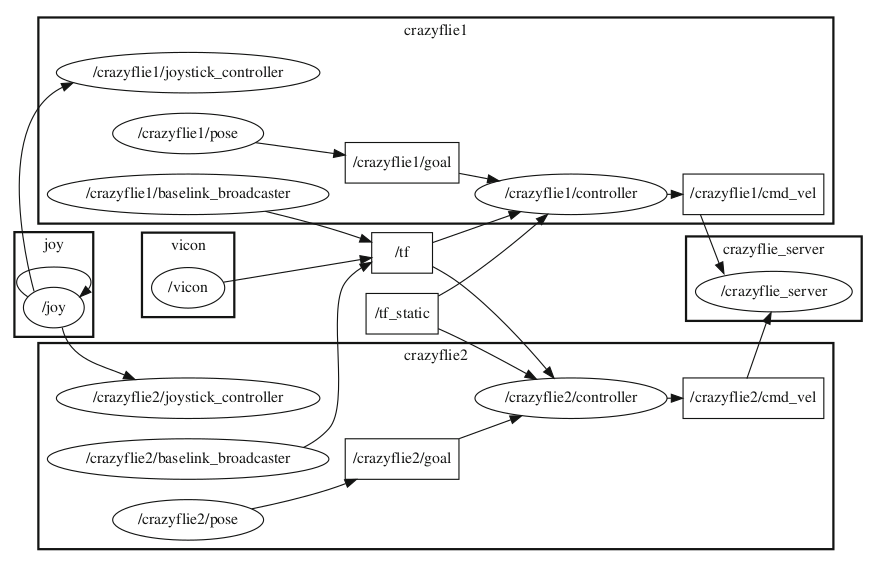
\includegraphics[scale=0.5]{Figures/hoenig_topics.png}
 \caption{ROS nodes, namespaces and topics used when controlling multiple as described in \cite{HoenigMixedReality2015}}
 \label{figure:hoenig_topics}
\end{figure}.

\subsection{Modifying the gps node to publish tf frames}
\label{section:servicelayer_gps_final}
\noindent What is of particular interest in this section is to publish drone tf frames by modifying the \texttt{servicelayer\_gps\_ros} package from \ref{listing:servicelayer_v1} instead of using the Vicon motion capture system. The modified source code can be seen in Listing \ref{listing:servicelayer_tf_frames} below:

\begin{code}
\begin{minted}[breaklines, linenos, frame=single]{cpp}
// SmartCity includes
#include <ros/ros.h>
#include <tf/transform_broadcaster.h>

// GPS.cpp code

DataStorage_t Data;
std::string cf_id;
std::string cf_frame;
std::string stream_port_str;
int stream_port;
std::string ip;
int frequency;
int server_port;
MarkerOffset_t marker_offset;

void publishTransform(const GPS_Data &pose)
{
    static tf::TransformBroadcaster br;
    tf::Transform transform;
    transform.setOrigin( tf::Vector3(pose.x, pose.y, pose.z) );
    tf::Quaternion q;
    q.setRPY(0, 0, pose.yaw);
    transform.setRotation(q);
    br.sendTransform(tf::StampedTransform(transform, ros::Time::now(), "world", cf_frame));
}

int main(int argc, char** argv)
{
  marker_offset = {0,0,0};
  frequency = 100;
  ip = "192.168.0.100";
  server_port = 11111;
  
  ros::init(argc, argv, "crazyflie_broadcaster");

  if (argc != 4)
  {
    ROS_ERROR("need crazyflie id, frame and stream port");
    return -1;
  }
  cf_id = argv[1];
  cf_frame = argv[2];
  stream_port_str = argv[3];

  stream_port = std::stoi( stream_port_str );  //default 55555
  Data.vehicleID << (uint8_t)(std::stoi( cf_id ));

  GPS * gps = new GPS(&Data, marker_offset, frequency, ip, server_port, stream_port);
  GPS_Data pose;

  ros::NodeHandle node;

  ros::Rate loop_rate(100);

  while (ros::ok())
  {
    pose = Data.GPS.pop();
    publishTransform(pose);

    ros::spinOnce();

    loop_rate.sleep();
  }
  return 0;
}
\end{minted}
\caption{The servicelayer\_gps modified to publish tf frames\\}
\label{listing:servicelayer_tf_frames}
\end{code}

\noindent The following code lines are explained in more detail:

\begin{minted}[breaklines, frame=single]{cpp}
  marker_offset = {0,0,0};
  frequency = 100;
  ip = "192.168.0.100";
  server_port = 11111;
\end{minted}
\noindent Here the default values to connect to the SmartCity Optitrack server are assigned.

\begin{minted}[breaklines, frame=single]{cpp}
  if (argc != 4){ROS_ERROR("need crazyflie id and frame and server port"); return -1;};
  cf_id = argv[1];
  cf_frame = argv[2];
  server_port_str = argv[3];
\end{minted}
\noindent The gps node takes the Optitrack RigidBody id as an argument this time. In addition it is possible to specify under which frame name to publish the crazyflie tf frame. Lastly a different server port can be specified to potentially allow more than one connection to the server. The program will exit with an error if any of these arguments aren't given.

\begin{minted}[breaklines, frame=single]{cpp}
  GPS * gps = new GPS(&Data, marker_offset, frequency, ip, server_port, stream_port);
\end{minted}
\noindent This creates a GPS object the same way as in Listing \ref{listing:servicelayer_v1} with the possibility of choosing a different stream port to connect to the server. This is because the Optitrack server allows clients to connect only on port 11111, represented by the \texttt{server\_port} variable. It should however allow specifying a different streaming port which is expected to be required if position data for more than one drone is to be obtained.

The next step is to publish the the Optitrack gps data as a tf frame, a task that is handled by the \texttt{publishTransform()} function. It takes the \textit{pose} variable containing the most recent gps data as argument and uses it to create a tf tranform and a broadcaster that publishes it as seen in lines 19-20 of Listing \ref{listing:servicelayer_tf_frames} above.

\begin{minted}[breaklines, frame=single]{cpp}
{
    transform.setOrigin( tf::Vector3(pose.x, pose.y, pose.z) );
}
\end{minted}
\noindent Here the transform is assigned the translational $x,y,z$ coordinates.

\begin{minted}[breaklines, frame=single]{cpp}
{
    tf::Quaternion q;
    q.setRPY(0, 0, pose.yaw);
    transform.setRotation(q);
}
\end{minted}
\noindent Next the attitude of the drone is assigned to the transform. An extra step needs to be performed as the tf transform require quaternions to describe the attitude. Therefore a quaternion object \textit{q} is created and next the quaternion internal method \textit{setRPY()} is used to define the attitude by converting Euler $roll, pitch, yaw$ angles into quaternions. The SmartCity Optitrack server does not report $roll$ and $pitch$ which is why those values are set to zero.

\begin{minted}[breaklines, frame=single]{cpp}
{
  br.sendTransform(tf::StampedTransform(transform, ros::Time::now(), "world", cf_frame));
}
\end{minted}

\noindent As a last step \texttt{publishTransform()} publishes the created transform which reports the position of the drone frame (named according to the specified \textit{cf\_frame} variable ) in relation to the static \textit{world} frame shown in Figure \ref{figure:smart_city_layout}.

\noindent Assuming these steps are performed in continuation of the ones described for Listing \ref{listing:servicelayer_v1} the only remaining step is to re-build the source code, namely:
\begin{mdframed}[backgroundcolor=light-gray, linecolor=light-gray]
\begin{verbatim}
$ cd ~/crazyflie_ws/
$ catkin_make
\end{verbatim}
\end{mdframed}

\noindent Now the node can be run the same as before, by issuing the following command:
\begin{mdframed}[backgroundcolor=light-gray, linecolor=light-gray]
\begin{verbatim}
$ rosrun servicelayer_gps_ros GPS 111 crazyflie1 111111
\end{verbatim}
\end{mdframed}
\noindent but instead of publishing data to the \texttt{/server\_data} topic a tf frame will be published instead, same as obtained from the VRPN client in section \ref{section:ws3}. One noticeable exception is that when \texttt{tf echo} is run , the displayed tf frame contains the expected values of the drone in the SmartCity layout, as it can be seen below:

\begin{mdframed}[backgroundcolor=light-gray, linecolor=light-gray]
\begin{verbatim}
$ rosrun tf tf_echo /world /crazyflie1
At time 1542987286.924
- Translation: [2.254, 1.711, 0.439]
- Rotation: in Quaternion [0.0, 0.0, 0.675, 0.738]
            in RPY (radian) [0.0, 0.0, 1.482]
            in RPY (degree) [0.0, 0.0, 84.894]
\end{verbatim}
\end{mdframed}

\noindent Having this frame available the next step is to perform a test flight for a single drone.

\subsection{Pre-flight setup}
Before the server is tested the crazyflies are put in the same place as shown in Figure \ref{figure:smart_city_layout} and it is ensured that the PC is connected to the same network as the Optitrack server via an ethernet cable. To ensure that all the required nodes are launched for autonomous fligh, a new launch file is created by following by using \textit{hover\_vrpn.launch} from the crazyflie ros stack as example.
\begin{mdframed}[backgroundcolor=light-gray, linecolor=light-gray]
\begin{verbatim}
$ cd ~/crazyflie_ws/src/crazyflie_ros/crazyflie_demo/launch
$ hover.launch
\end{verbatim}
\end{mdframed}

\noindent to which the following content is added:
\begin{code}
\begin{minted}[breaklines, linenos, frame=single]{xml}
<?xml version="1.0"?>
<launch>
  <arg name="joy_dev" default="/dev/input/js0" />

  <arg name="uri" default="radio://0/100/2M/E7E7E7E701" />
  <arg name="frame" default="crazyflie1" />
  <arg name="x" default="3.5" />
  <arg name="y" default="0.8" />
  <arg name="z" default="0.4" />
  
  <arg name="cf_id" default="111" />
  <arg name="stream_port" default="11111" />

  <include file="$(find crazyflie_driver)/launch/crazyflie_server.launch">
  </include>

  <group ns="crazyflie">
    <include file="$(find crazyflie_driver)/launch/crazyflie_add.launch">
      <arg name="uri" value="$(arg uri)" />
      <arg name="tf_prefix" value="crazyflie" />
    </include>

    <node name="joy" pkg="joy" type="joy_node" output="screen">
      <param name="dev" value="$(arg joy_dev)" />
    </node>

    <node name="joystick_controller" pkg="crazyflie_demo" type="controller.py" output="screen">
      <param name="use_crazyflie_controller" value="True" />
    </node>

    <include file="$(find crazyflie_controller)/launch/crazyflie2.launch">
      <arg name="frame" value="$(arg frame)" />
    </include>

    <node name="pose" pkg="crazyflie_demo" type="publish_pose.py" output="screen">
      <param name="name" value="goal" />
      <param name="rate" value="30" />
      <param name="x" value="$(arg x)" />
      <param name="y" value="$(arg y)" />
      <param name="z" value="$(arg z)" />
    </node>

    <node pkg="tf" type="static_transform_publisher" name="baselink_broadcaster" args="0 0 0 0 0 0 1 $(arg frame) /crazyflie/base_link 100" />
    
    <!-- run servicelayer_gps_ros -->
    <node name="gps" pkg="servicelayer_gps_ros" type="GPS" args="$(arg cf_id) $(arg frame) $(arg stream_port)" />
    
  </group>
</launch>

\end{minted}
\end{code}

\noindent What is changed from the default launch file is that the custom servicelayer node is run on line 46 is the above listing instead of the vicon or the VRPN node. The arguments given to it are equivalent to running \texttt{rosrun servicelayer\_gps\_ros} as shown in subsection \ref{section:servicelayer_gps_final} except that there is no need to launch all nodes separately as the launch file runs all the required components.\\
An important part of this launch file is to specify the desired setpoint for the drone to reach, namely $x, y, z$ coordinates in the SmartCity layout. Since hover is desired for this test, the $x$ and $y$ starting position are specified depending on where the drone is located and the $z$ coordinate is given in this case at a height of 0.4 meters (line 9 in the above Listing)

\subsection{Test flight - single crazyflie}
At this point it is possible to perform a test flight by making a single drone hover about given $x, y, z$ coordinates. The drone is placed on the ground in the SmartCity layout and it is ensured that the current $x,y$ coordinates of the drone are set in the \textit{hover.launch} file and the gamepad and the CrazyRadio PA are connected to the PC. The following command is issued:
\begin{mdframed}[backgroundcolor=light-gray, linecolor=light-gray]
\begin{verbatim}
$ roslaunch crazyflie_demo hover.launch
\end{verbatim}
\end{mdframed}

\noindent Once the above command is run, press initiate the "takeoff" command by pressing the respective button on the gamepad (the "O" button is the default for PS3/PS4 gamepads).
At this point the drone should take off and eventually settle around the hover point. Figure \ref{figure:plot_hover_single} below shows the actual $z$ position of the drone starting with the takeoff command and time zero. Around the 27th second mark the "Land" command, by pressing, in this the "square" button on the gamepad.

\begin{figure}[H]
\centering
 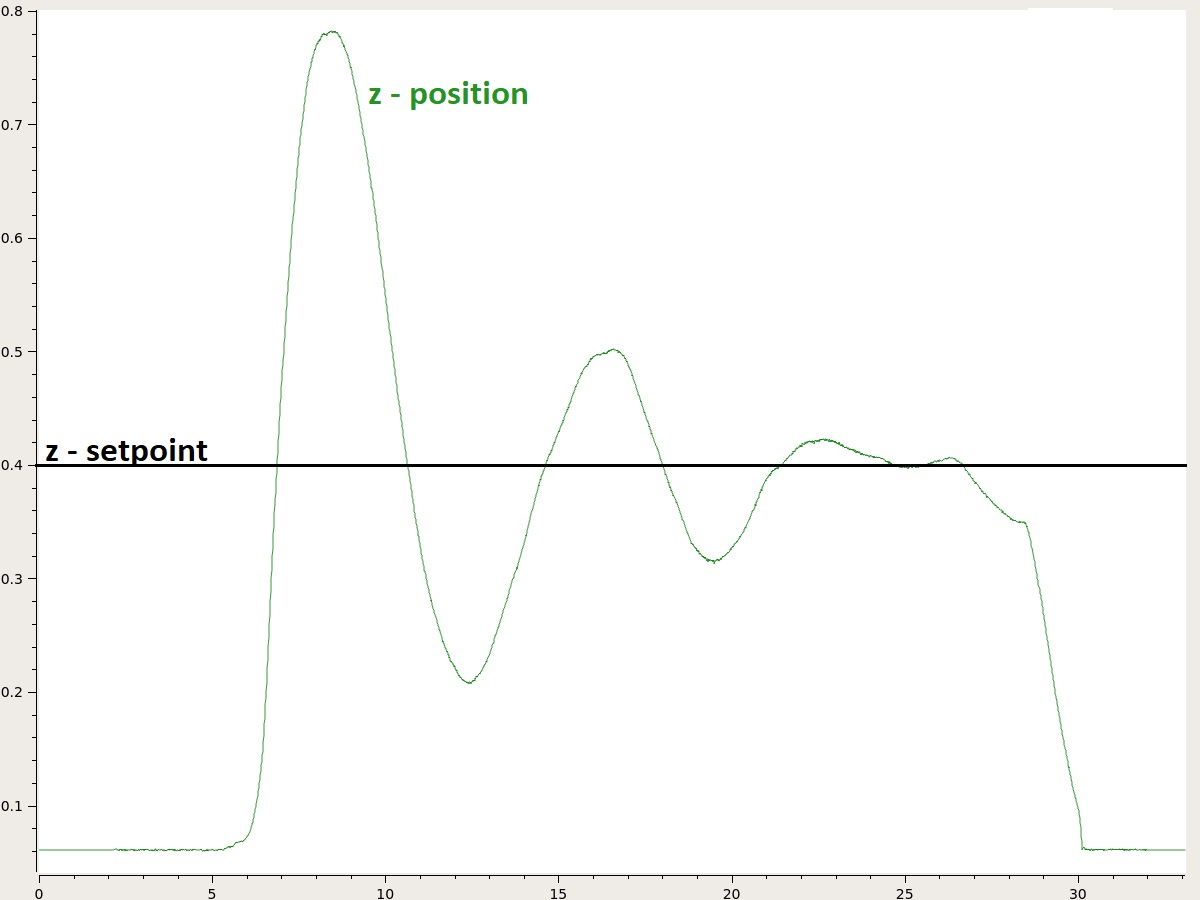
\includegraphics[scale=0.25]{Figures/hover_single.jpg}
 \caption{Plotted z position of the drone when commanded to hover at the 0.4 meter point on the z-axis}
 \label{figure:plot_hover_single}
\end{figure}.

The drone is able to hover at around the 0.4 meters height and observing the flight behaviour it is able to do so with minor deviations. It can maintain this state for up to 7 minutes as the battery runs out. The next section attempts to hover 2 Crazyflie drones at the same time.
